\documentclass[11pt,a4paper]{article}
\usepackage[utf8]{inputenc}
\usepackage{geometry}
\geometry{a4paper, margin=1in}
\usepackage{tikz}
\usetikzlibrary{positioning, shapes.geometric, arrows.meta, fit, backgrounds, calc}
\usepackage{hyperref}
\usepackage{booktabs}
\usepackage{titlesec}
\usepackage{xcolor}
\usepackage{tabularx}

\title{Domain-Driven Design: FitSync Platform}
\author{}
\date{}

\begin{document}
\maketitle

\tableofcontents
\newpage

\section{Project Description}
FitSync is a comprehensive multi-tenant platform designed to bridge the gap between fitness enthusiasts, trainers, gym owners, and fitness product sellers. The platform supports multiple user roles: Trainee, Trainer, Gym Owner, Seller, Manager, and Admin, each with specific workflows. Trainees can discover gyms, buy memberships, book trainers, and purchase fitness gear. Gym owners and sellers manage their respective businesses, including gym listings, trainer associations, and product inventories.

\section{Domain-Driven Design}
We structured the FitSync platform using Domain-Driven Design (DDD) principles. The entire domain is broken down into four bounded contexts, where each one covers a specific area of business logic with its own boundaries, entities, value objects, and domain services.

\subsection{Bounded Contexts}
The system is logically divided into four primary Bounded Contexts.

\vspace{1em}
\noindent
\begin{tabularx}{\textwidth}{l X}
\toprule
\textbf{BOUNDED CONTEXT} & \textbf{RESPONSIBILITY / KEY DOMAIN CONCEPTS} \\
\midrule
\textbf{Identity \& Access} & Handles user registration, authentication, role-based profiles, and user metrics. \newline \textit{Concepts: User, Profile, Role, AuthToken} \\
\midrule
\textbf{Gym Operations} & Manages gym listings, facilities, pricing, trainers associated with the gym, and analytics for gym owners. \newline \textit{Concepts: Gym, Location, Pricing, Schedule, Analytics} \\
\midrule
\textbf{Membership \& Training} & Handles the lifecycle of gym memberships, trainer-trainee assignments, and training progress tracking. \newline \textit{Concepts: GymMembership, TrainerAssignment, TrainerProgress, BillingDetails} \\
\midrule
\textbf{E-commerce} & Manages physical products, shopping carts, orders, order items, and product reviews. \newline \textit{Concepts: Order, Product, Cart, ProductReview, ShippingAddress} \\
\bottomrule
\end{tabularx}

\vspace{1.5em}
\begin{center}
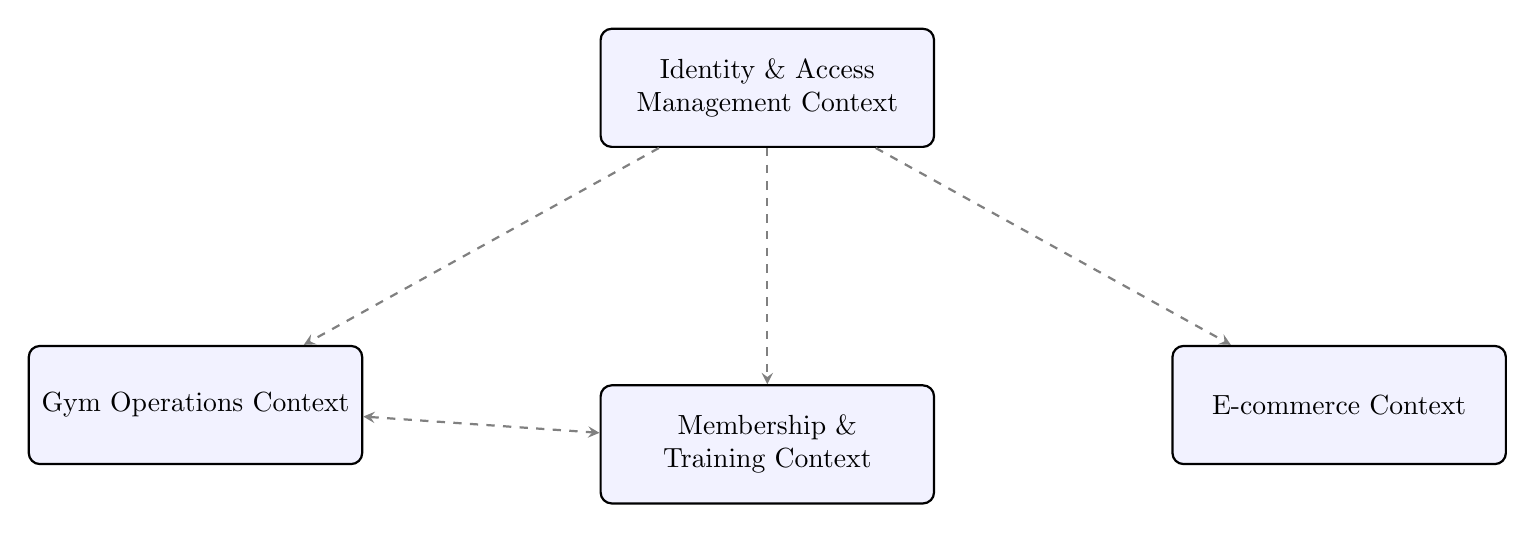
\begin{tikzpicture}[
    node distance=2.5cm and 3cm,
    context/.style={rectangle, rounded corners, draw=black, thick, text width=4cm, align=center, minimum height=1.5cm, fill=blue!5}
]
    \node[context] (iam) {Identity \& Access Management Context};
    \node[context] (gym) [below left=of iam] {Gym Operations Context};
    \node[context] (ecommerce) [below right=of iam] {E-commerce Context};
    \node[context] (membership) [below=3cm of iam] {Membership \& Training Context};

    \draw[dashed, ->, >=stealth, thick, gray] (iam) -- (gym);
    \draw[dashed, ->, >=stealth, thick, gray] (iam) -- (ecommerce);
    \draw[dashed, ->, >=stealth, thick, gray] (iam) -- (membership);
    \draw[dashed, <->, >=stealth, thick, gray] (gym) -- (membership);
\end{tikzpicture}
\end{center}

\subsection{Context Mappings}
Context maps lay out how the different bounded contexts relate to each other and how they exchange data.

\vspace{1em}
\noindent
\begin{tabularx}{\textwidth}{l l l X}
\toprule
\textbf{UPSTREAM} & \textbf{DOWNSTREAM} & \textbf{PATTERN} & \textbf{DESCRIPTION} \\
\midrule
Identity & Gym Operations & Shared Kernel & The User entity (as Owner/Trainer) is referenced by Gym. IAM owns identity and shares it. \\
\midrule
Identity & E-commerce & Shared Kernel & The User (as Buyer/Seller) places orders and lists products. \\
\midrule
Identity & Membership & Shared Kernel & Memberships are tied to Trainee and Trainer User entities. \\
\midrule
Gym & Membership & Partnership & Membership relies heavily on Gym entities to define the subscribed facilities. \\
\bottomrule
\end{tabularx}

\subsection{Entities, Value Objects \& Services}

\subsubsection*{1. Identity \& Access Management Context}
\noindent
\begin{tabularx}{\textwidth}{l l X}
\toprule
\textbf{TYPE} & \textbf{NAME} & \textbf{KEY ATTRIBUTES / RESPONSIBILITY} \\
\midrule
Entity & User & name, email, password, role, status, profile, metrics, refreshToken \\
Value Object & Profile & headline, about, location, company, socialLinks \\
Value Object & Role & Enum: user, trainee, trainer, gym-owner, seller, manager, admin \\
Value Object & Metrics & ownerMetrics, traineeMetrics, trainerMetrics \\
Service & AuthService & Register, login, token generation, password hashing \\
\bottomrule
\end{tabularx}

\subsubsection*{2. Gym Operations Context}
\noindent
\begin{tabularx}{\textwidth}{l l X}
\toprule
\textbf{TYPE} & \textbf{NAME} & \textbf{KEY ATTRIBUTES / RESPONSIBILITY} \\
\midrule
Entity & Gym & name, description, owner (ref), trainers (ref), status, approvalStatus \\
Value Object & Location & address, city, state, postalCode, coordinates \\
Value Object & Pricing & monthlyMrp, monthlyPrice, currency \\
Value Object & Schedule & openTime, closeTime, workingDays \\
Value Object & Contact & phone, email, website, whatsapp \\
Service & GymService & CRUD gyms, status updates, search and filter \\
\bottomrule
\end{tabularx}

\subsubsection*{3. Membership \& Training Context}
\noindent
\begin{tabularx}{\textwidth}{l l X}
\toprule
\textbf{TYPE} & \textbf{NAME} & \textbf{KEY ATTRIBUTES / RESPONSIBILITY} \\
\midrule
Entity & GymMembership & trainee (ref), gym (ref), trainer (ref), plan, startDate, endDate, status \\
Entity & TrainerAssignment & trainee (ref), trainer (ref), status, schedule \\
Value Object & BillingDetails & amount, currency, paymentGateway, status \\
Service & MembershipService & Subscription lifecycle, renewal, billing updates \\
\bottomrule
\end{tabularx}

\subsubsection*{4. E-commerce Context}
\noindent
\begin{tabularx}{\textwidth}{l l X}
\toprule
\textbf{TYPE} & \textbf{NAME} & \textbf{KEY ATTRIBUTES / RESPONSIBILITY} \\
\midrule
Entity & Order & buyer (ref), seller (ref), totalAmount, status, paymentMethod \\
Entity & Product & seller (ref), name, description, price, stock, category \\
Entity & Cart & user (ref), items[], totalAmount \\
Value Object & OrderItem & product (ref), name, quantity, price, status \\
Value Object & ShippingAddress & name, address, city, state, zipCode, phone \\
Service & OrderService & Order creation, status tracking, payment flow \\
\bottomrule
\end{tabularx}

\subsection{Cardinality Ratios}

\vspace{1em}
\noindent
\begin{tabularx}{\textwidth}{l c X}
\toprule
\textbf{RELATIONSHIP} & \textbf{CARDINALITY} & \textbf{CONSTRAINT / NOTES} \\
\midrule
User to Gym (Owner) & 1:N & An owner can have multiple gyms \\
User to Gym (Trainer) & M:N & Trainers can be associated with multiple gyms \\
User to Order (Buyer) & 1:N & A buyer can place many orders \\
User to Product (Seller) & 1:N & A seller manages multiple products \\
User to Cart & 1:1 & Each user has one active cart \\
Gym to GymMembership & 1:N & A gym has many active memberships \\
Order to OrderItem & 1:N & An order contains multiple line items \\
\bottomrule
\end{tabularx}

\subsection{Aggregates}
Aggregates set the consistency boundaries within the domain. Each aggregate has a root entity that acts as the single point of access.

\vspace{1.5em}
\begin{center}
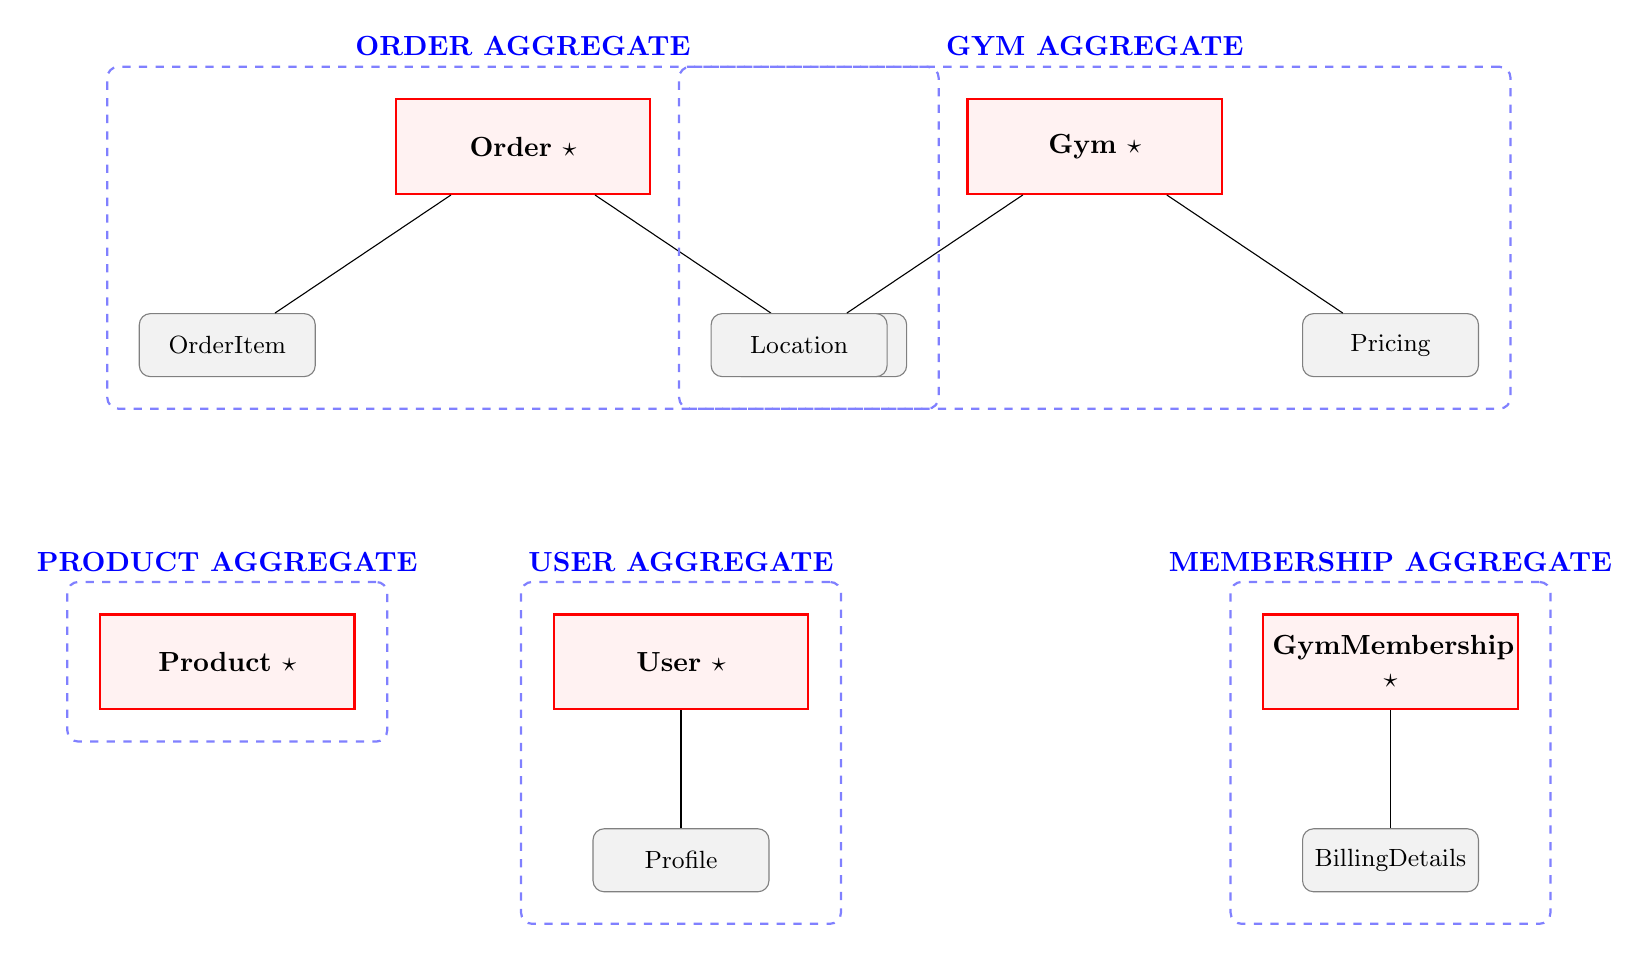
\begin{tikzpicture}[
    node distance=1.5cm and 1cm,
    entity/.style={rectangle, draw=black, thick, fill=white, text width=2.5cm, align=center, minimum height=1cm},
    vo/.style={rectangle, draw=gray, rounded corners, fill=gray!10, text width=2cm, align=center, minimum height=0.8cm, font=\small},
    root/.style={rectangle, draw=red, thick, fill=red!5, text width=3cm, align=center, minimum height=1.2cm, font=\bfseries},
    aggregate/.style={draw=blue!50, thick, dashed, inner sep=0.4cm, rounded corners}
]

    % Order Aggregate
    \node[root] (order) {Order $\star$};
    \node[vo] (orderitem) [below left=of order] {OrderItem};
    \node[vo] (address) [below right=of order] {Address};
    \draw[-] (order) -- (orderitem);
    \draw[-] (order) -- (address);
    \node[aggregate, fit=(order) (orderitem) (address), label=above:\textcolor{blue}{\textbf{ORDER AGGREGATE}}] (orderAgg) {};

    % Gym Aggregate
    \node[root] (gym) [right=4cm of order] {Gym $\star$};
    \node[vo] (location) [below left=of gym] {Location};
    \node[vo] (pricing) [below right=of gym] {Pricing};
    \draw[-] (gym) -- (location);
    \draw[-] (gym) -- (pricing);
    \node[aggregate, fit=(gym) (location) (pricing), label=above:\textcolor{blue}{\textbf{GYM AGGREGATE}}] (gymAgg) {};

    % Product Aggregate
    \node[root] (product) [below=3cm of orderitem] {Product $\star$};
    \node[aggregate, fit=(product), label=above:\textcolor{blue}{\textbf{PRODUCT AGGREGATE}}] (prodAgg) {};

    % Membership Aggregate
    \node[root] (membership) [below=3cm of pricing] {GymMembership $\star$};
    \node[vo] (billing) [below=of membership] {BillingDetails};
    \draw[-] (membership) -- (billing);
    \node[aggregate, fit=(membership) (billing), label=above:\textcolor{blue}{\textbf{MEMBERSHIP AGGREGATE}}] (memAgg) {};

    % User Aggregate
    \node[root] (user) [right=2.5cm of product] {User $\star$};
    \node[vo] (profile) [below=of user] {Profile};
    \draw[-] (user) -- (profile);
    \node[aggregate, fit=(user) (profile), label=above:\textcolor{blue}{\textbf{USER AGGREGATE}}] (userAgg) {};

\end{tikzpicture}
\end{center}

\end{document}
